\begin{refsection}

\chapter{U--Pb}
\label{ch:UPb-R}

\noindent\begin{minipage}[t]{.5\linewidth}
\strut\vspace*{-\baselineskip}\newline
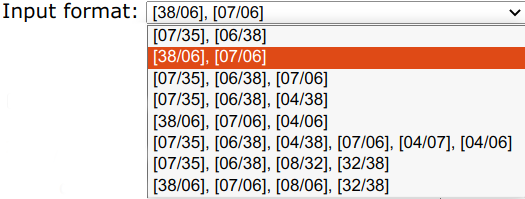
\includegraphics[width=\linewidth]{../figures/UPbFormats.png}\\
\end{minipage}
\begin{minipage}[t]{.5\textwidth}
  \texttt{IsoplotR} accommodates eight U--Pb formats. See
  Section~\ref{sec:UPbFormats} for details.
\end{minipage}

\noindent Examples using the CLI:

\begin{script}
# U-Pb format 1, 1se absolute input errors:
UPb1 <- read.data('UPb1.csv',method='U-Pb',format=1)
# U-Pb format 6, 1se relative input errors:
UPb2 <- read.data('UPb6.csv',method='U-Pb',format=6,ierr=3)
# U-Pb format 8, 2se relative input errors:
UPb3 <- read.data('UPb8.csv',method='U-Pb',format=8,ierr=4)
\end{script}

\noindent where \texttt{UPb1.csv}, \texttt{UPb6.csv} and
\texttt{UPb8.csv} are files that, like the example files of
Section~\ref{ch:generic-R}, are included in \texttt{IsoplotR} and
whose file path can be found with the \texttt{system.file()} function.\\

\noindent\begin{minipage}[t]{.15\linewidth}
\strut\vspace*{-\baselineskip}\newline
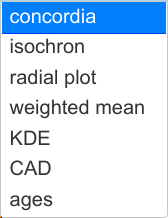
\includegraphics[width=\linewidth]{../figures/UPbPlotdevices.png}
\end{minipage}
\begin{minipage}[t]{.85\textwidth}
  U--Pb data can be visualised on five or six different plot devices
  and output tables. The \texttt{isochron} option is only available
  for formats 4--8 and is hidden otherwise. See the remaining sections
  of this chapter for examples of these output options.
\end{minipage}

\section{General options}
\label{sec:general}

\begin{enumerate}

  \item\label{it:UPbLambdairatio} Isotopic ratios and decay constants:

\noindent\begin{minipage}[t]{.6\linewidth}
\strut\vspace*{-\baselineskip}\newline
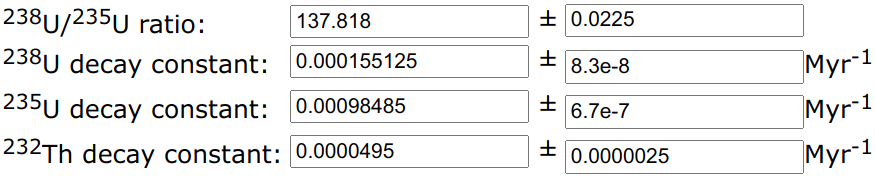
\includegraphics[width=\linewidth]{../figures/UPbLambda.png}
\end{minipage}
\begin{minipage}[t]{.4\linewidth}
  The default \textsuperscript{238}U/\textsuperscript{235}U ratio is
  given by \citet{hiess2012}, and the U and Th decay constants by
  \citet{jaffey1971} and \citet{leroux1963}, respectively.
\end{minipage}

\begin{script}
# use the Steiger and Jaeger (1977) value with zero uncertainty
settings('iratio','U238U235',137.88,0)
# use the Schoene et al. (2006) value and uncertainty
settings('lambda','U238',0.000154993,0.00000013) 
\end{script}

\item\label{it:common-Pb-concordia} Common Pb correction of the
  individual aliquots can be carried out using the methods of
  Section~\ref{sec:common-Pb}. This may be useful for single grain
  analysis tools such as the KDE, CAD, radial or weighted mean
  plot. For cogenetic aliquots that form an isochron, the common Pb is
  best left uncorrected. In this case the most reliable age estimate
  is given by the isochron through the uncorrected data, which can be
  visualised on a concordia diagram (Section~\ref{sec:concordia-R}) or
  (for formats 4--8) as a separate isochron plot
  (Section~\ref{sec:UPb-isochron-R}).\\

\noindent\begin{minipage}[t]{.4\linewidth}
\strut\vspace*{-\baselineskip}\newline
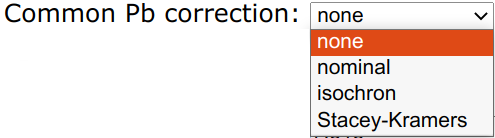
\includegraphics[width=\linewidth]{../figures/CommonPb.png}
\end{minipage}
\begin{minipage}[t]{.6\linewidth}
  A common Pb menu is available for all output types except
  \texttt{isochron}. It gives access to four different common Pb
  treatments that can be applied to the data before plotting.
\end{minipage}

\begin{enumerate}
\item\begin{minipage}[t]{.4\linewidth}
  \strut\vspace*{-\baselineskip}\newline
  
\includegraphics[width=\linewidth]{../figures/nominalcommonpb.png}
  \end{minipage}
  \begin{minipage}[t]{.6\linewidth}
    Selecting the \texttt{nominal} option implements the common Pb
    correction algorithm of
    Section~\ref{sec:common-Pb}.\ref{it:nominalcommonpb}.\\
  \end{minipage}

  \noindent\begin{minipage}[t]{.43\linewidth}
  \strut\vspace*{-\baselineskip}\newline
  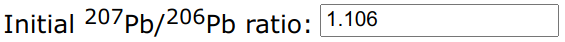
\includegraphics[width=\linewidth]{../figures/initialPb76.png}
  \end{minipage}
  \begin{minipage}[t]{.57\linewidth}
    If \texttt{nominal} has been selected, and the data are of formats
    1--3, a new text box appears with the
    \textsuperscript{207}Pb/\textsuperscript{206}Pb ratio of the
    common Pb.\\
  \end{minipage}

\begin{script}
settings('iratio','Pb207Pb206',1.106)
radialplot(UPb1,common.Pb=1)
\end{script}

  \noindent\begin{minipage}[t]{.4\linewidth}
  \strut\vspace*{-\baselineskip}\newline
  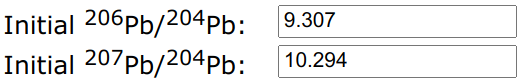
\includegraphics[width=\linewidth]{../figures/initialPb764.png}
  \end{minipage}
  \begin{minipage}[t]{.6\linewidth}
    For U--Pb data formats 4--6, the nominal common Pb composition is specified
    as a pair of \textsuperscript{206}Pb/\textsuperscript{204}Pb and 
    \textsuperscript{207}Pb/\textsuperscript{204}Pb ratios.\\
  \end{minipage}

\begin{script}
settings('iratio','Pb206Pb204',9.307)
settings('iratio','Pb207Pb204',10.294)
weightedmean(UPb2,common.Pb=1)
\end{script}

  \noindent\begin{minipage}[t]{.42\linewidth}
  \strut\vspace*{-\baselineskip}\newline
  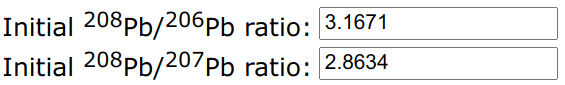
\includegraphics[width=\linewidth]{../figures/initialPb876.png}
  \end{minipage}
  \begin{minipage}[t]{.58\linewidth}
    Finally, for U--Pb data formats 7 and 8, the nominal common Pb
    composition is specified as a pair of
    \textsuperscript{208}Pb/\textsuperscript{206}Pb and
    \textsuperscript{208}Pb/\textsuperscript{207}Pb ratios.\\
  \end{minipage}

\begin{script}
settings('iratio','Pb208Pb206',3.1671)
settings('iratio','Pb208Pb207',2.8634)
weightedmean(UPb3,common.Pb=1)
\end{script}

\item\noindent\begin{minipage}[t]{.4\linewidth}
  \strut\vspace*{-\baselineskip}\newline
  
\includegraphics[width=\linewidth]{../figures/isochroncommonpb.png}
  \end{minipage}
  \begin{minipage}[t]{.6\linewidth}
    Selecting the \texttt{isochron} option implements the common Pb
    correction algorithm of
    Section~\ref{sec:common-Pb}.\ref{it:isochroncommonpb}. In other
    words, it projects all the aliquots parallel to the isochron and
    onto the radiogenic dimension. It is important to reiterate that
    selecting this option does \textbf{not} return the isochron age!
  \end{minipage}
  
\begin{script}
kde(UPb2,common.Pb=2)
\end{script}
  
\item\noindent\begin{minipage}[t]{.4\linewidth}
  \strut\vspace*{-\baselineskip}\newline
  
\includegraphics[width=\linewidth]{../figures/staceykramerscommonpb.png}
  \end{minipage}
  \begin{minipage}[t]{.6\linewidth}
    Selecting the \texttt{Stacey-Kramers} option implements the common
    Pb correction algorithm of
    Section~\ref{sec:common-Pb}.\ref{it:separate-stacey-kramers}.
  \end{minipage}

\begin{script}
cad(UPb1,common.Pb=3)
\end{script}

\end{enumerate}

\item Initial disequilibrium can be activated by ticking the
  corresponding box in the GUI, or by calling the \texttt{diseq()}
  function from the CLI. The output of the latter function must be
  called from the \texttt{read.data()} function.

\noindent\begin{minipage}[t]{.6\linewidth}
  \strut\vspace*{-\baselineskip}\newline
  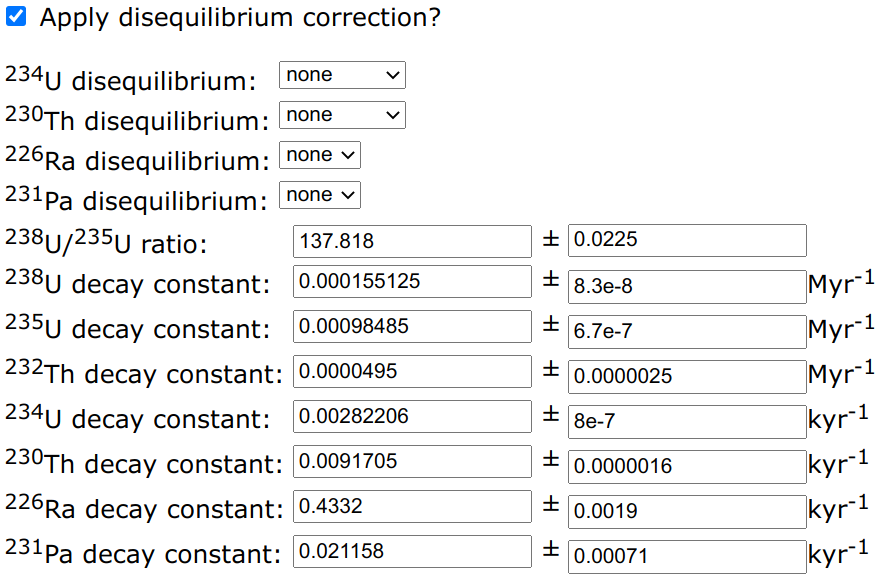
\includegraphics[width=\linewidth]{../figures/UPbDisequilibriumSettings.png}
  \end{minipage}
  \begin{minipage}[t]{.4\linewidth}
    Ticking the initial disequilibrium box reveals the decay constants
    of \textsuperscript{234}U, \textsuperscript{230}Th,
    \textsuperscript{226}Ra and \textsuperscript{231}Pa.  From the
    CLI, these parameters can be changed using the \texttt{settings()}
    function in exactly the same way as shown in
    Section~\ref{sec:general}.\ref{it:UPbLambdairatio}.
  \end{minipage}

\begin{enumerate}

\item There are two ways to specify the initial disequilibrium
  conditions for \textsuperscript{234}U and \textsuperscript{230}Th:
  
\noindent\begin{minipage}[t]{.6\linewidth}
  \strut\vspace*{-\baselineskip}\newline
  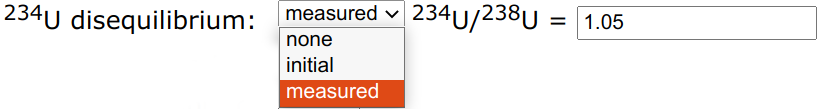
\includegraphics[width=\linewidth]{../figures/U234-disequilibrium.png}
  \end{minipage}
  \begin{minipage}[t]{.4\linewidth}
If the sample is young enough that secular equilibrium has not yet
been re-established, then any measured remanent disequilibrium can be
specified here.
  \end{minipage}

\noindent CLI example:
\begin{script}
d <- diseq(U48=list(x=1.05,option=2))
UPb4 <- read.data('diseq.csv',method='U-Pb',format=2,d=d)
concordia(UPb4,type=2)
\end{script}

\item For the shortest lived isotopes \textsuperscript{226}Ra and
  \textsuperscript{231}Pa, only one option is available:
  
\noindent\begin{minipage}[t]{.6\linewidth}
  \strut\vspace*{-\baselineskip}\newline
  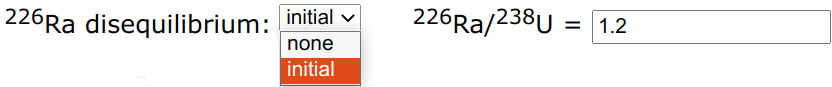
\includegraphics[width=\linewidth]{../figures/Ra226-disequilibrium.png}
\end{minipage}
\begin{minipage}[t]{.4\linewidth}
It is generally not possible to measure the remanent disequilibrium
for these isotopes, so the only option is to specify the hypothesised
initial activity ratio.
\end{minipage}

\noindent CLI example:
\begin{script}
d <- diseq(RaU=list(x=1.2,option=1))
UPb4 <- read.data('diseq.csv',method='U-Pb',format=2,d=d)
concordia(UPb4,type=2)
\end{script}

\item Finally, for U--Pb data of formats 7 and 8 (which include the
  \texttt{232}Th/\textsuperscript{238}U ratio of the mineral), there
  is a fourth way to specify the initial
  \textsuperscript{230}Th/\textsuperscript{238}U activity ratio, by
  supplying the measured Th/U-ratio of the magma, determined by
  geochemical analysis of the whole rock or volcanic glass:

\noindent\begin{minipage}[t]{.6\linewidth}
    \strut\vspace*{-\baselineskip}\newline
    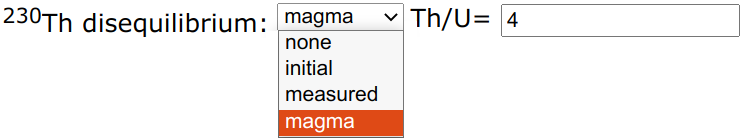
\includegraphics[width=\linewidth]{../figures/Th230-disequilibrium.png}
  \end{minipage}
  \begin{minipage}[t]{.4\linewidth}
    \texttt{IsoplotR} combines this measured ratio with the
    \textsuperscript{232}Th/\textsuperscript{238}U-ratio of the
    minerals to compute the Th/U fractionation factor.
  \end{minipage}

\noindent CLI example:
\begin{script}
d <- diseq(ThU=list(x=3,option=3))
UPb4 <- read.data('diseq.csv',method='U-Pb',format=8,d=d)
radialplot(UPb4)
\end{script}

\end{enumerate}

The different disequilibrium settings can be combined in the GUI, and
from the command line using the \texttt{diseq} function:

\begin{script}
d <- diseq(U48=list(x=0,option=1),ThU=list(x=2,option=1),
           RaU=list(x=2,option=1),PaU=list(x=2,option=1))
UPb4 <- read.data('diseq.csv',method='U-Pb',format=2,d=d)
concordia(UPb4,type=2,xlim=c(0,5000),ylim=c(0.047,0.057))
\end{script}

\end{enumerate}

\section{Concordia} \label{sec:concordia-R}

\noindent\begin{minipage}[t]{.3\linewidth}
  \strut\vspace*{-\baselineskip}\newline
  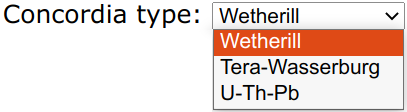
\includegraphics[width=\linewidth]{../figures/ConcordiaMenu.png}
\end{minipage}
\begin{minipage}[t]{.7\linewidth}
  \texttt{IsoplotR} offers three types of concordia diagrams. The
  U--Th--Pb diagram is only available for U--Pb data formats 7 and 8.
\end{minipage}

\begin{script}
concordia(UPb1,type=1) # Wetherill
concordia(UPb1,type=2) # Tera-Wasserburg
concordia(UPb3,type=3) # U-Th-Pb
\end{script}

\begin{enumerate}

\item The limits of the concordia diagram can be specified in two
  ways:

  \noindent\begin{minipage}[t]{.4\linewidth}
  \strut\vspace*{-\baselineskip}\newline
  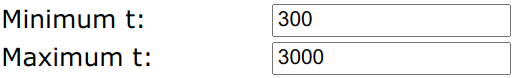
\includegraphics[width=\linewidth]{../figures/Concordiatlim.png}
\end{minipage}
\begin{minipage}[t]{.6\linewidth}
  The first option is to specify the minimum and maximum age of the
  concordia line.
\end{minipage}

\begin{script}
# Wetherill diagram from 300 to 3000 Ma:
concordia(UPb1,tlim=c(300,3000)) 
\end{script}

\noindent\begin{minipage}[t]{.4\linewidth}
  \strut\vspace*{-\baselineskip}\newline
  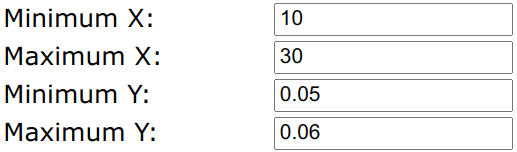
\includegraphics[width=\linewidth]{../figures/ConcordiaXYlim.png}
\end{minipage}
\begin{minipage}[t]{.6\linewidth}
  Alternatively, the limits of the concordia diagram can also be
  specified by the minimum and maximum extent of the horizontal and
  vertical axis.
\end{minipage}

\begin{script}
# Tera-Wasserburg diagram with U238/Pb206 limits from 10 to 30
# and Pb207/Pb206 limits from 0.05 to 0.06:
concordia(UPb1,type=2,xlim=c(10,30),ylim=c(0.05,0.06))
\end{script}

\item By default, \texttt{IsoplotR} plots error ellipses and
  calculates confidence intervals at a 95\% confidence level.

  \noindent\begin{minipage}[t]{.4\linewidth}
  \strut\vspace*{-\baselineskip}\newline
  
\includegraphics[width=\linewidth]{../figures/ConcordiaAlpha.png}
\end{minipage}
\begin{minipage}[t]{.6\linewidth}
To plot the data as `2 sigma' ellipses, this can be changed to
$\alpha=0.14$ here, which covers 86\% of the area under a bivariate
normal distribution:
\end{minipage}

\begin{console}
concordia(UPb1,alpha=0.14)
\end{console}

\item When an extra variable is entered in the optional \texttt{(C)}
  column of the input table, this can be used as a colour scale (see
  Section~\ref{sec:GUI}).

  \noindent\begin{minipage}[t]{.4\linewidth}
  \strut\vspace*{-\baselineskip}\newline
  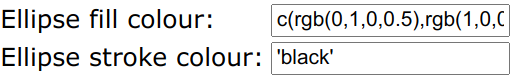
\includegraphics[width=\linewidth]{../figures/ConcordiaColours.png}
\end{minipage}
\begin{minipage}[t]{.6\linewidth}
  The corresponding fill and stroke colours can be specified by
  entering \texttt{R} code in the text box of the GUI.\\
\end{minipage}

\noindent To illustrate the different possibilities, let us consider a
U--Pb dataset of format~7 or 8 and use the Th/U ratios to build a
colour scale:
\begin{console}
ThU <- UPb3$x$Th232U238
\end{console}

\noindent Specify the fill colours by name:
\begin{console}
concordia(UPb3,levels=ThU,ellipse.fill=c('blue','red'))
\end{console}

\noindent Using red-green-blue-transparency (rgb-alpha) specifiers:
\begin{console}
concordia(UPb3,levels=ThU,ellipse.fill=c(rbg(1,0,0,0.5),rgb(0,1,0,0.5)))
\end{console}

\noindent Specifying the stroke colours as a colour palette with 80\% opacity
and using a uniform white colour for the fill colour:
\begin{script}
concordia(UPb3,levels=ThU,ellipse.fill='white',
          ellipse.stroke=heat.colors(n=10,alpha=0.8))
\end{script}

\noindent Leaving the error ellipses empty but using a reversed colour palette
for the stroke colour:
\begin{console}
concordia(UPb3,levels=ThU,ellipse.fill=NA,ellipse.stroke=rev(rainbow(n=10)))
\end{console}

\noindent\begin{minipage}[t]{.4\linewidth}
\strut\vspace*{-\baselineskip}\newline

\includegraphics[width=\linewidth]{../figures/UPbColourLabel.png}
\end{minipage}
\begin{minipage}[t]{.6\linewidth}
  Specifying colour levels adds a colour bar to the concordia diagram,
  which can be labelled for clarity.
\end{minipage}

\begin{console}
concordia(UPb3,levels=ThU,clabel='Th/U')
\end{console}

\item \texttt{IsoplotR} automatically chooses a `pretty' sequence of
  age ticks for the concordia line.

  \noindent\begin{minipage}[t]{.4\linewidth}
  \strut\vspace*{-\baselineskip}\newline
  
\includegraphics[width=\linewidth]{../figures/Concordiatticks.png}
\end{minipage}
\begin{minipage}[t]{.6\linewidth}
  These default values can be overruled by a comma separated list of
  numerical values (in Myr).
\end{minipage}

\begin{console}
concordia(UPb1,ticks=c(230,240,250))
\end{console}

Alternatively, the \texttt{ticks} argument can also be used to simply
specify the number of ticks:

\begin{console}
concordia(UPb1,ticks=10)
\end{console}

\item Labelling the error ellipses can be useful to identify outliers
  or otherwise noteworthy aliquots.

  \noindent\begin{minipage}[t]{.25\linewidth}
  \strut\vspace*{-\baselineskip}\newline
  
\includegraphics[width=\linewidth]{../figures/concordiashownumbers.png}
\end{minipage}
\begin{minipage}[t]{.75\linewidth}
  Ticking the box labels the ellipses with the row numbers of the
  input data.
\end{minipage}

\begin{console}
concordia(UPb1,show.numbers=TRUE)
\end{console}

\item Besides a data visualisation device, the concordia diagram can
  also be used as a vehicle for various numerical calculations:

\noindent\begin{minipage}[t]{.3\linewidth}
  \strut\vspace*{-\baselineskip}\newline
  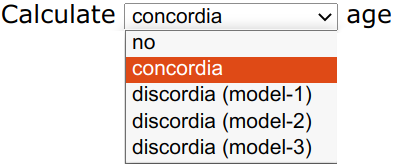
\includegraphics[width=\linewidth]{../figures/ConcordiaShowAge.png}
\end{minipage}
\begin{minipage}[t]{.7\linewidth}
  Selecting the \texttt{concordia} option adds a white ellipse with
  the concordia composition to the plot, as well as a legend with the
  concordia age, confidence intervals, MSWD and p-values.
\end{minipage}

Compute the concordia age of the first 9 aliquots. Show the
10\textsuperscript{th} aliquot but do not use it for the calculation:

\begin{console}
concordia(UPb1,show.age=1,omit=10)
\end{console}

\item Decay constant uncertainties can be visualised as a thicker
  concordia line, and propagated into any derived numerical values.

\noindent\begin{minipage}[t]{.35\linewidth}
\strut\vspace*{-\baselineskip}\newline

\includegraphics[width=\linewidth]{../figures/concordiaexterr.png}
\end{minipage}
\begin{minipage}[t]{.65\linewidth}
  Ticking the box adds the decay constant (and
  \textsuperscript{238}U/\textsuperscript{235}U ratio) uncertainty
  after the concordia composition has been calculated.
\end{minipage}

The following code snippet does not only omit the
10\textsuperscript{th} aliquot from the calculation, but also removes
it from the plot altogether. The external uncertainties are added by
the optional \texttt{exterr} argument:

\begin{console}
concordia(UPb1,show.age=1,hide=10,exterr=TRUE)
\end{console}

\item \texttt{IsoplotR} implements three discordia regression models,
  as discussed in Section~\ref{sec:discordia}.

  \noindent\begin{minipage}[t]{.3\linewidth}
  \strut\vspace*{-\baselineskip}\newline
  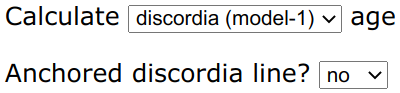
\includegraphics[width=\linewidth]{../figures/discordia.png}
  \end{minipage}
  \begin{minipage}[t]{.7\linewidth}
    By default the discordia regression is unconstrained so that both
    the age and common Pb composition of cogenetic aliquots can be
    simultaneously estimated.\\
  \end{minipage}

  \noindent Visualising a model-1 fit in three dimensions on a
  Tera-Wasserburg concordia diagram, which returns the isochron age
  and common Pb composition:
\begin{console}
concordia(UPb2,type=2,show.age=2)
\end{console}

\noindent Model-2 regression of the same data visualised on a
Wetherill concordia diagram, which reports the upper and lower age
intercept:
\begin{console}
concordia(UPb2,type=1,show.age=3)
\end{console}

\item The discordia line can also be anchored to a particular common
  Pb composition.
  
  \noindent\begin{minipage}[t]{.3\linewidth}
  \strut\vspace*{-\baselineskip}\newline
  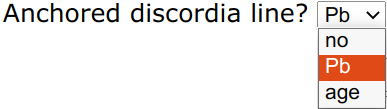
\includegraphics[width=\linewidth]{../figures/anchoreddiscordia.png}
  \end{minipage}
  \begin{minipage}[t]{.7\linewidth}
For formats 1--3, the common Pb anchored is specified via a
\textsuperscript{207}Pb/\textsuperscript{206}Pb value. For formats
4--6, it is specified via a pair of
\textsuperscript{206}Pb/\textsuperscript{204}Pb and
\textsuperscript{207}Pb/\textsuperscript{204}Pb values, and for
formats~7 and 8, via the initial
\textsuperscript{206}Pb/\textsuperscript{208}Pb and
\textsuperscript{207}Pb/\textsuperscript{208}Pb values.    
  \end{minipage}

\noindent Specifying the common Pb composition is done in exactly the
same way as the common Pb corrections of
Section~\ref{sec:general}.\ref{it:common-Pb-concordia}. For example:

\begin{script}
settings('iratio','Pb206Pb204',9.307)
settings('iratio','Pb207Pb204',10.294)
concordia(UPb2,type=2,show.age=3,anchor=1)
\end{script}

\item Alternatively, the discordia line can also be anchored to a
  particular age intercept.

\noindent\begin{minipage}[t]{.4\linewidth}
\strut\vspace*{-\baselineskip}\newline

\includegraphics[width=\linewidth]{../figures/discordiaageanchor.png}
\end{minipage}
\begin{minipage}[t]{.6\linewidth}
  Selecting the \texttt{age} option adds a text box to the GUI in
  which the age anchor can be specified (in Ma).
\end{minipage}

From the CLI:
\begin{console}
concordia(UPb2,type=2,show.age=3,anchor=c(2,300))
\end{console}

\item The number of significant digits can be specified relative to
  the analytical uncertainty. For example, if \texttt{sigdig}=2, then
  $123.45678 \pm 0.12345$ is rounded to $123.46 \pm 0.12$.

\noindent\begin{minipage}[t]{.4\linewidth}
\strut\vspace*{-\baselineskip}\newline

\includegraphics[width=\linewidth]{../figures/sigdig.png}
\end{minipage}
\begin{minipage}[t]{.6\linewidth}
  The significant digits affect all numerical output that is reported
  in the figure legend.
\end{minipage}

Reporting model-3 discordia regression results to 3 significant
digits:
\begin{console}
concordia(UPb2,show.age=4,sigdig=3)
\end{console}

\end{enumerate}

\section{Isochrons} \label{sec:UPb-isochron-R}

The option to visualise U--Pb data as isochrons is only available for
data formats 4--8.

\begin{enumerate}

  \item For formats 4--6, \textsuperscript{204}Pb is used as a
    normalising isotope
    (Section~\ref{sec:discordia}.\ref{it:UPbIsochron46}).

\noindent\begin{minipage}[t]{.3\linewidth}
\strut\vspace*{-\baselineskip}\newline
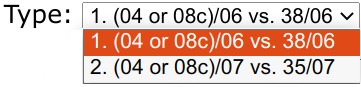
\includegraphics[width=\linewidth]{../figures/UPbIsochron.png}
\end{minipage}
\begin{minipage}[t]{.7\linewidth}
Either \textsuperscript{206}Pb or \textsuperscript{207}Pb can be used
as the radiogenic isotope.
\end{minipage}

\noindent Using the CLI to create a two-panel plot of
\textsuperscript{204}Pb-based isochron diagrams:
\begin{script}
oldpar <- par(mfrow=c(1,2))
isochron(UPb2,type=1) # 204Pb/206Pb vs. 238U/206Pb
isochron(UPb2,type=2) # 204Pb/207Pb vs. 235U/207Pb
par(oldpar)
\end{script}

\item U--Th--Pb isochrons for formats~7 and 8 can be visualised in
  four different ways. Let \textsuperscript{208}Pb\textsubscript{c},
  \textsuperscript{207}Pb\textsubscript{c} and
  \textsuperscript{206}Pb\textsubscript{c} be the
  \textsuperscript{208}Pb, \textsuperscript{207}Pb and
  \textsuperscript{206}Pb component with the radiogenic component
  removed. Then these non radiogenic components can be used as a
  normalising isotope for the U- and Th-decay systems.

\noindent\begin{minipage}[t]{.3\linewidth}
\strut\vspace*{-\baselineskip}\newline
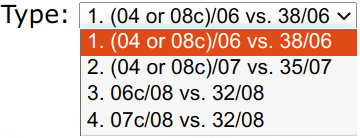
\includegraphics[width=\linewidth]{../figures/UPbFormats78isochronMenu.png}
\end{minipage}
\begin{minipage}[t]{.7\linewidth}
  \textsuperscript{208}Pb\textsubscript{c} is used as a normalising
  isotope for the uranium clock, and
  \textsuperscript{206}Pb\textsubscript{c} or
  \textsuperscript{207}Pb\textsubscript{c} for the thorium clock.
\end{minipage}
  
\noindent Using the CLI to create a ${2}\times{2}$ grid of isochron
diagrams:
\begin{script}
oldpar <- par(mfrow=c(2,2))
isochron(UPb3,type=1) # 208Pbc/206Pb vs. 238U/206Pb
isochron(UPb3,type=2) # 208Pbc/207Pb vs. 235U/207Pb
isochron(UPb3,type=3) # 206Pbc/208Pb vs. 232Th/208Pb
isochron(UPb3,type=4) # 207Pbc/208Pb vs. 232Th/208Pb
par(oldpar)
\end{script}

\item \noindent\begin{minipage}[t]{.45\linewidth}
  \strut\vspace*{-\baselineskip}\newline
  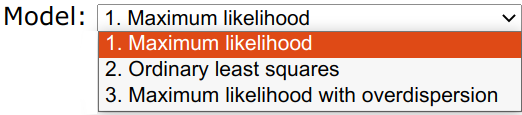
\includegraphics[width=\linewidth]{../figures/UPbIsochronModels.png}
\end{minipage}
\begin{minipage}[t]{.55\linewidth}
  The same three regression models that were available for discordia
  regression under the \texttt{concordia} function are also available
  under the \texttt{isochron} function.  In fact, their numerical
  output is exactly the same.
\end{minipage}

\noindent $2\times{2}$ grid of CLI examples:
\begin{console}
oldpar <- par(mfrow=c(2,2))
# model-3 regression of 204Pb/206Pb vs. 238U/206Pb:
isochron(UPb2,type=1,model=3)
# model-2 regression of 204Pb/207Pb vs. 235U/207Pb:
isochron(UPb2,type=2,model=2)
# model-1 regression of 208Pbc/206Pb vs. 238U/206Pb:
isochron(UPb3,type=2,model=1)
# model-3 regression of 207Pbc/208Pb vs. 232Th/208Pb:
isochron(UPb3,type=3,model=3)
par(oldpar)
\end{console}

\item \noindent\begin{minipage}[t]{.4\linewidth}
  \strut\vspace*{-\baselineskip}\newline
  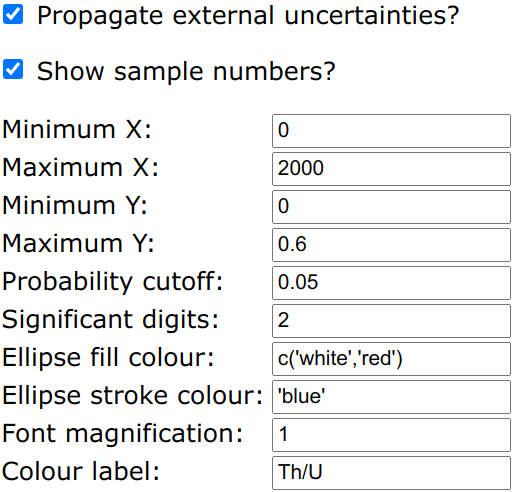
\includegraphics[width=\linewidth]{../figures/UPbIsochronExtraOptions.png}\\
\end{minipage}
  \begin{minipage}[t]{.6\linewidth}
    The output of the \texttt{isochron} function can be modified using
    many of the same optional arguments as the \texttt{concordia}
    function.  Thus, we can change the horizontal (\texttt{xlim}) and
    vertical (\texttt{ylim}) extent of the plot, adjust the number of
    significant digits (\texttt{sigdig}), modify the significance
    level (\texttt{alpha}) of the numerical results and error
    ellipses, label the error ellipses with the sample numbers
    (\texttt{show.numbers}), propagate the decay constant
    uncertainties \texttt{exterr}, and label the and colour those
    ellipses (\texttt{ellipse.fill} and \texttt{ellipse.stroke})
    according to some additional variable \texttt{levels}.
\end{minipage}
From the CLI, we can also store the results of the isochron regression
in a variable for further processing. For example:
\begin{script}
ThU <- UPb3$x$Th232U238
fit <- isochron(UPb3,type=3,model=1,xlim=c(0,2000),ylim=c(0,0.5),
                alpha=0.1,sigdig=3,show.numbers=TRUE,levels=ThU,
                ellipse.fill=c('white','red'),ellipse.stroke='blue',
                clabel='Th/U')
\end{script}

\end{enumerate}

\section{Radial plots}
\label{sec:UPbRadial}

\begin{enumerate}

\item The radial plot is a graphical device to display single grain
  ages. \texttt{IsoplotR} offers five ways to computer single grain
  U--Pb ages, as discussed in
  Section~\ref{sec:discfilter}. Additionally, for U--Pb data formats~7
  and 8, it also adds the option to plot the data as
  \textsuperscript{208}Pb/\textsuperscript{232}Th ages:

\noindent\begin{minipage}[t]{.35\linewidth}
  \strut\vspace*{-\baselineskip}\newline
  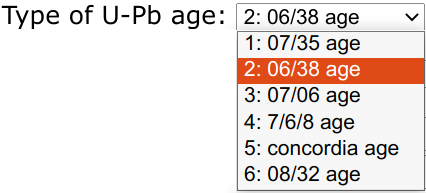
\includegraphics[width=\linewidth]{../figures/UPbRadialAgeTypes.png}
\end{minipage}
\begin{minipage}[t]{.65\linewidth}
  The default option is to calculate single grain concordia ages. In
  this screenshot, that is changed to
  \textsuperscript{206}Pb/\textsuperscript{238}U ages.
\end{minipage}

\begin{console}
radialplot(UPb1,type=2)
\end{console}

\noindent\begin{minipage}[t]{.35\linewidth}
  \strut\vspace*{-\baselineskip}\newline
  
\includegraphics[width=\linewidth]{../figures/UPbRadial678age.png}
\end{minipage}
\begin{minipage}[t]{.65\linewidth}
  The \texttt{6/7/8 age} option applies the
  \textsuperscript{206}Pb/\textsuperscript{238}U method to young ages
  and the \textsuperscript{207}Pb/\textsuperscript{206}Pb method to
  old ages.
\end{minipage}

\noindent\begin{minipage}[t]{.4\linewidth}
  \strut\vspace*{-\baselineskip}\newline
  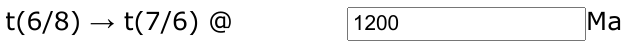
\includegraphics[width=\linewidth]{../figures/UPbRadial678switch.png}
\end{minipage}
\begin{minipage}[t]{.6\linewidth}
  When the \texttt{6/7/8 age} option is selected, a new text box
  appears in which the user can specify when to switch between the two
  methods.
\end{minipage}

\begin{console}
radialplot(UPb1,type=4,cutoff.76=1200)
\end{console}

\item A discordance filter can be applied to the U--Pb data prior to
  the construction of the radial plot:
  
  \noindent\begin{minipage}[t]{.5\linewidth}
  \strut\vspace*{-\baselineskip}\newline
  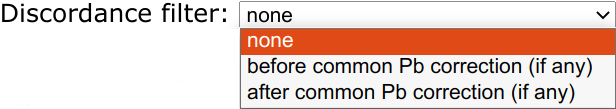
\includegraphics[width=\linewidth]{../figures/UPbRadialDiscfilter.png}\\
\end{minipage}
  \begin{minipage}[t]{.5\linewidth}
    For formats 4--8, the discordance filter can be applied either
    before or after the common Pb correction.
  \end{minipage}

For formats 1--3, the discordance filter can only be applied before
the common Pb correction, because this correction forces all the data
to be perfectly concordant (see Section~\ref{sec:common-Pb}). The
\texttt{before common Pb correction (if any)} and \texttt{after common
  Pb correction (if any)} options will only produce a different result
if a common Pb correction option is applied, as discussed in
Section~\ref{sec:general}.\ref{it:common-Pb-concordia}. Five
discordance filters are available, as discussed in
Section~\ref{sec:discfilter}:
\begin{center}
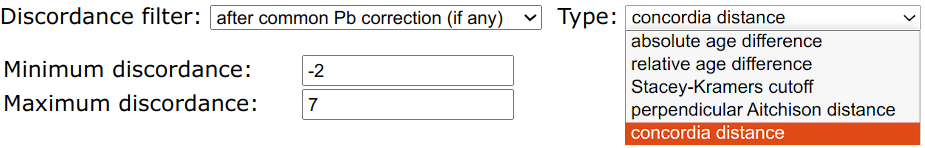
\includegraphics[width=.9\linewidth]{../figures/UPbRadialConcordiaDiscfilter.png}
\end{center}
\noindent CLI examples:

\noindent Apply a $-2$ to $+7$\% concordia distance filter without common
  Pb correction:
\begin{console}
radialplot(UPb1,cutoff.disc=discfilter(option=5,cutoff=c(-2,7)))
\end{console}

\noindent Apply a $-5$ to $+15$\% relative age filter after a
  isochron-based common Pb correction:
\begin{script}
dscf <- cutoff.disc=discfilter(option=2,before=FALSE,cutoff=c(-5,15))
radialplot(UPb2,common.Pb=2,cutoff.disc=dscf)
\end{script}

\noindent Apply a $0$ to $+1$\% Stacey-Kramers filter after a nominal
  common Pb correction:
\begin{script}
settings('iratio','Pb208Pb206',2.089)
settings('iratio','Pb208Pb207',2.519)
dscf <- cutoff.disc=discfilter(option=3,before=FALSE,cutoff=c(0,1))
radialplot(UPb3,common.Pb=1,cutoff.disc=dscf)
\end{script}

\noindent Apply a $-1$ to $+5$\% perpendicular Aitchison filter before a
  Stacey-Kramers based common Pb correction:
\begin{script}
dscf <- cutoff.disc=discfilter(option=4,before=TRUE,cutoff=c(-1,5))
radialplot(UPb3,common.Pb=3,cutoff.disc=dscf)
\end{script}

\item Just like concordia diagrams and isochron plots, also radial
  plots can be modified using various optional formatting arguments
  (Section~\ref{sec:OtherRadial}).

\noindent\begin{minipage}[t]{.45\linewidth}
\strut\vspace*{-\baselineskip}\newline
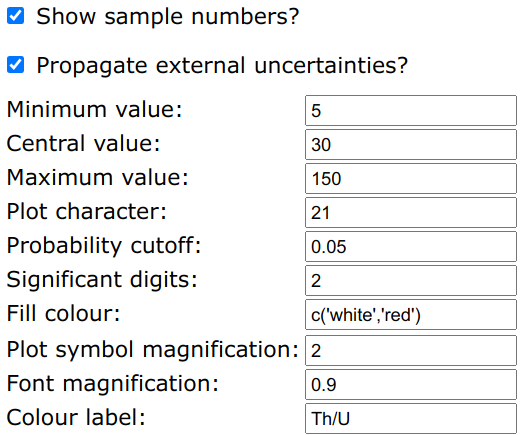
\includegraphics[width=\linewidth]{../figures/UPbRadialOtherOptions.png}
\end{minipage}
\begin{minipage}[t]{.55\linewidth}
  The minimum and maximum extent of the radial scale can be specified,
  as well as the central value ($z_\circ$ in
  Equation~\ref{eq:radial}). Samples are represented by filled circles
  by default, but this can be changed to a range of other shape. These
  can be specified as numbers (\texttt{1-25}, see \texttt{?pch} for
  further details) or a single character such as \verb|'o'|,
  \verb|'*'|, \verb|'+'|, or \verb|'.'|. For plot characters that have
  a fill colour (e.g., \texttt{21-25}), an additional variable can be
  used to construct a colour scale. Both the plot symbols and any text
  labels in the plot of legend can be magnified or reduced via a
  scaling factor.
\end{minipage}

\begin{script}
oldpar <- par(pch=0.9) # font magnification
radialplot(UPb3,show.numbers=TRUE,exterr=TRUE,from=5,z0=30,to=150,
           pch=21,alpha=0.05,bg=c('white','red'),cex=2,
           levels=UPb3$x$Th232U238,clabel='Th/U')
par(oldpar)
\end{script}

\end{enumerate}

\section{Weighted mean}
\label{sec:UPbWtdMean}

The weighted mean plot serves a similar purpose as the radial plot and
shares several options with it.

\noindent\begin{minipage}[t]{.5\linewidth}
\strut\vspace*{-\baselineskip}\newline
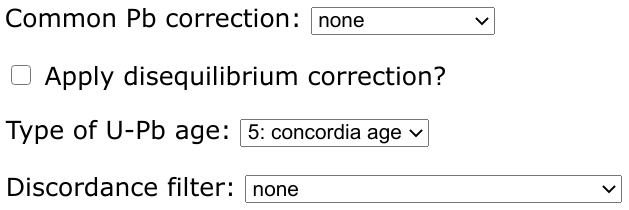
\includegraphics[width=\linewidth]{../figures/UPbWtdMeanAgeType.png}
\end{minipage}
\begin{minipage}[t]{.5\linewidth}
  Like the radial plot, also the weighted mean function can be
  applied to five or six different types of U--(Th)--Pb dates. These
  may or may not be corrected for common Pb and initial
  disequilibrium, and may or may not have passed through a discordance
  filter.
\end{minipage}

Using the default settings:
\begin{console}
weightedmean(UPb1)
\end{console}

A more sophisticated example showing the disequilibrium corrected
\textsuperscript{206}Pb/\textsuperscript{238}U dates with a concordia
distance age filter (with default limits from $-2$\% to $+7$\%) that
is applied before a Stacey--Kramer common Pb correction:

\begin{script}
d <- diseq(U48=list(x=0,option=1),ThU=list(x=2,option=1),
           RaU=list(x=2,option=1),PaU=list(x=2,option=1))
UPb4 <- read.data('diseq.csv',method='U-Pb',format=2,d=d)
weightedmean(UPb4,type=2,common.Pb=3,cutoff.disc=discfilter(option=5))
\end{script}

The remaining options of the weighted mean function are the same as
for the generic version discussed in
Section~\ref{sec:OtherWeightedMean}.\\

\noindent\begin{minipage}[t]{.4\linewidth}
\strut\vspace*{-\baselineskip}\newline
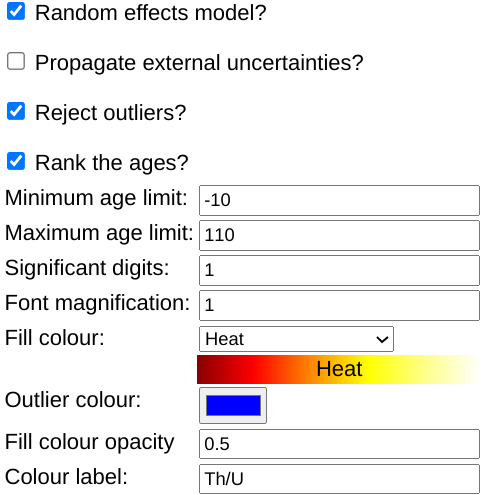
\includegraphics[width=\linewidth]{../figures/UPbWeightedMeanOtherOptions.png}
\end{minipage}
\begin{minipage}[t]{.6\linewidth}
  The ages can be averaged either using the one-parameter ordinary
  weighted mean algorithm, or the two-parameter random effects
  algorithm.  Outliers are detected using the modified Chauvenet
  criterion, which may select different outliers for the ordinary
  weighted mean and random effects model.  By default the aliquots are
  plotted in the order of the input table. However they can also be
  shuffled in order of increasing age.  The minimum and maximum extent
  of the age scale can be specified and may extend to negative values;
  the fill colour of the rectangular segments can be modified based on
  an additional variable, with a designated separate colour for
  outliers; the confidence level and significant digits can be
  specified as in the concordia, isochron and radial plots.
\end{minipage}

\begin{script}
weightedmean(UPb3,random.effects=TRUE,detect.outliers=TRUE,
             outlier.col='red',ranked=TRUE,from=-10,to=100,
             alpha=0.02,sigdig=1,levels=UPb3$x$Th232U238,
             rect.col=rev(topo.colors(n=100)),clabel='Th/U')
\end{script}

\section{Kernel density estimates}
\label{sec:UPbKDE}

Like the radial plot and weighted mean plot, also the kernel density
estimation function can be applied to five or six different types of
U--(Th)--Pb dates.

\noindent\begin{minipage}[t]{.5\linewidth}
\strut\vspace*{-\baselineskip}\newline
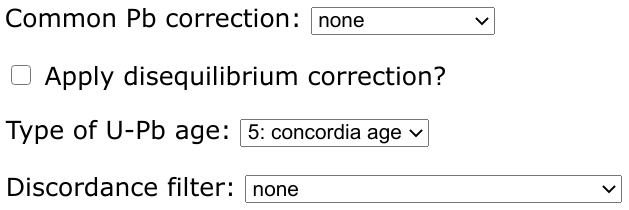
\includegraphics[width=\linewidth]{../figures/UPbWtdMeanAgeType.png}
\end{minipage}
\begin{minipage}[t]{.5\linewidth}
 The U--Pb data may or may not be corrected for common Pb and initial
 disequilibrium, and may or may not have passed through a discordance
 filter.
\end{minipage}

\begin{script}
d <- discfilter(option=4,before=FALSE,cutoff=c(-1,5))
kde(UPb2,common.Pb=2,type=2,cutoff.disc=d)
\end{script}

All other options are as in Section~\ref{sec:OtherKDE}.

\section{Cumulative age distributions}
\label{sec:UPbCAD}

Like the radial, weighted mean and KDE plots, also the CAD can be used
to visualise five or six (depending on the U--Pb data format)
different U--Pb ages.\\

\noindent\begin{minipage}[t]{.5\linewidth}
\strut\vspace*{-\baselineskip}\newline
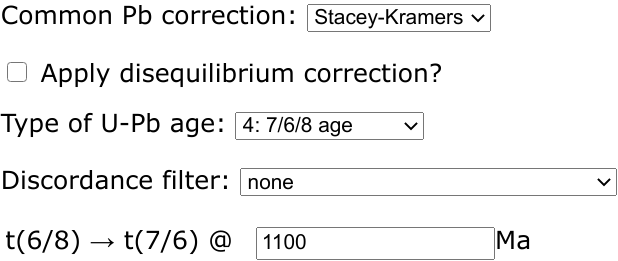
\includegraphics[width=\linewidth]{../figures/UPbCADageTypes.png}
\end{minipage}
\begin{minipage}[t]{.5\linewidth}
  And like these other diagrams, the data can corrected for initial
  disequilibrium or common Pb and filtered for discordance prior to
  visualisation as a CAD.
\end{minipage}

\begin{console}
cad(UPb1,common.Pb=3,type=4,cutoff.76=1100)
\end{console}

All other options are as in Section~\ref{sec:OtherCAD}.

\section{Ages}\label{sec:UPbAges}

Besides plotting diagrams, \texttt{IsoplotR} can also generate data
tables, which can be downloaded as \texttt{.csv} files. For U--Pb data
formats 1--6, these tables contain the
\textsuperscript{207}Pb/\textsuperscript{235}U,
\textsuperscript{206}Pb/\textsuperscript{238}U,
\textsuperscript{207}Pb/\textsuperscript{206}Pb and single grain
concordia ages. For formats 7 and 8, the
\textsuperscript{208}Pb/\textsuperscript{232}Th age is also reported.
In addition to this, there is also the option to add a column with the
estimate discordance of each aliquot.

\begin{enumerate}

\item Each aliquot can be corrected for initial disequilibrium or
  common Pb.

\noindent\begin{minipage}[t]{.4\linewidth}
\strut\vspace*{-\baselineskip}\newline

\includegraphics[width=\linewidth]{../figures/UPbAgesPb0diseq.png}
\end{minipage}
\begin{minipage}[t]{.6\linewidth}
  Note that, for formats 1--3, the common Pb correction always
  produces perfectly concordant ages. Which may not be the most
  informative result.
\end{minipage}

\begin{console}
age(UPb2,common.Pb=3)
\end{console}

\item The decay constant uncertainties can be added to each age.

\noindent\begin{minipage}[t]{.35\linewidth}
\strut\vspace*{-\baselineskip}\newline

\includegraphics[width=\linewidth]{../figures/UPbAgesExterr.png}
\end{minipage}
\begin{minipage}[t]{.65\linewidth}
  Note that the uncertainties of the resulting ages may be strongly
  correlated.
\end{minipage}
  
\begin{console}
age(UPb1,exterr=TRUE)
\end{console}

\item An additional column can be added to the output table listing
  the estimated discordance for each aliquot, which can either be
  calculated before or after the common Pb correction.
  \begin{center}
  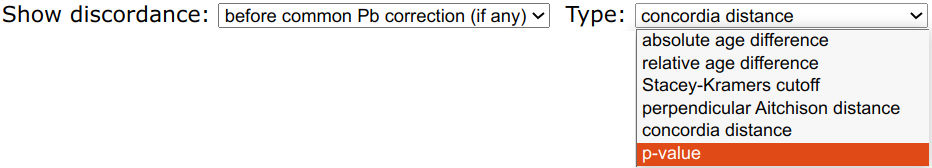
\includegraphics[width=.85\linewidth]{../figures/UPbAgesDiscordance.png}
  \end{center}
  In addition to the six discordance filter options that were
  available to the radial, weighted mean, KDE and CAD plots, the ages
  function also adds the option to list the p-value for concordance of
  each aliquot. Although this value should not be used as a basis to
  filter data, it may be useful for other purposes.
  
\begin{console}
age(UPb3,common.Pb=3,discordance=discfilter(before=TRUE,option=6))
\end{console}

\item The numerical results can be reported to any number of
  significant digits.

\noindent\begin{minipage}[t]{.4\linewidth}
\strut\vspace*{-\baselineskip}\newline

\includegraphics[width=\linewidth]{../figures/UPbAgesSigdig.png}
\end{minipage}
\begin{minipage}[t]{.6\linewidth}
  This may be useful if the results are to be used for subsequent
  calculations.
\end{minipage}

\begin{console}
tt <- age(UPb1,sigdig=4)
\end{console}

\end{enumerate}

\printbibliography[heading=subbibliography]

\end{refsection}
